\let\negmedspace\undefined
\let\negthickspace\undefined
\documentclass[journal]{IEEEtran}
\usepackage[a5paper, margin=10mm, onecolumn]{geometry}
%\usepackage{lmodern} % Ensure lmodern is loaded for pdflatex
\usepackage{tfrupee} % Include tfrupee package

\setlength{\headheight}{1cm} % Set the height of the header box
\setlength{\headsep}{0mm}     % Set the distance between the header box and the top of the text

\usepackage{gvv-book}
\usepackage{gvv}
\usepackage{cite}
\usepackage{amsmath,amssymb,amsfonts,amsthm}
\usepackage{algorithmic}
\usepackage{graphicx}
\usepackage{textcomp}
\usepackage{xcolor}
\usepackage{txfonts}
\usepackage{listings}
\usepackage{enumitem}
\usepackage{mathtools}
\usepackage{gensymb}
\usepackage{comment}
\usepackage[breaklinks=true]{hyperref}
\usepackage{tkz-euclide} 
\usepackage{listings}
% \usepackage{gvv}                                        
\def\inputGnumericTable{}                                 
\usepackage[latin1]{inputenc}                                
\usepackage{color}                                            
\usepackage{array}                                            
\usepackage{longtable}                                       
\usepackage{calc}                                             
\usepackage{multirow}                                         
\usepackage{hhline}                                           
\usepackage{ifthen}                                           
\usepackage{lscape}
\begin{document}

\bibliographystyle{IEEEtran}
\vspace{3cm}

\title{CHAPTER - 16\\Probability}
\author{EE24BTECH11061 - Rohith Sai}
% \maketitle
% \newpage
% \bigskip
{\let\newpage\relax\maketitle}

\renewcommand{\thefigure}{\theenumi}
\renewcommand{\thetable}{\theenumi}
\setlength{\intextsep}{10pt} % Space between text and floats

\numberwithin{figure}{enumi}
\renewcommand{\thetable}{\theenumi}

\section*{Exercise : 16.3}
\begin{enumerate}
\item [8.1)] Three coins are tossed once, what is the probability of getting three heads?\\
\textbf{Solution: }\\
Define a discrete random variable X = number of heads\newline
We will take our random variable as a sum of outcomes of three Bernoulli random variables
\begin{align}
\quad X = X_1+X_2+X_3
\end{align}
Where
\begin{align}
X_i = 
\begin{cases}
\quad 1, & \text{Outcome in Heads}\\
\quad 0, & \text{Outcome in Tails}
\end{cases}\\
p_{X_i}(n) = 
\begin{cases}
\quad 1-p, & n = 0\\
\quad p, & n = 1
\end{cases}
\end{align}
Where $p=\frac{1}{2}$\newline
Using properties of Z-Transform of PMF
\begin{align}
\quad M_X(z) &= M_{X_1}(z)M_{X_2}(z)M_{X_3}(z)\\
\quad M_{X_1}(z) &= \sum_{n=-\infty}^{\infty}p_{X_1}(n)z^{-n} = (1-p)+pz^{-1}\\
\quad M_{X_2}(z) &= \sum_{n=-\infty}^{\infty}p_{X_2}(n)z^{-n} = (1-p)+pz^{-1}\\
\quad M_{X_3}(z) &= \sum_{n=-\infty}^{\infty}p_{X_3}(n)z^{-n} = (1-p)+pz^{-1}\\
\quad M_X(z) &= ((1-p)+pz^{-1})^3\\
\quad &= \sum_{n=-\infty}^{\infty}\comb{3}{n}(1-p)^{3-n}p^nz^{-n}\\
\quad p_{X}(n) &= \comb{3}{n}p^{n}(1-p)^{3-n}\\
\quad p_{X}(n) &= \frac{\comb{3}{n}}{8}
\end{align}
The Probability Mass Function (PMF) for the given random variable is
\begin{align}
\quad p_X(n) =
\begin{cases}
\quad \frac{1}{8}, & n = 0 \\
\quad \frac{3}{8}, & n = 1 \\
\quad \frac{3}{8}, & n = 2 \\
\quad \frac{1}{8}, & n = 3 \\
\end{cases}
\end{align}
The probability of getting three heads is
\begin{align}
\quad p_X(3) = \frac{1}{8}
\end{align}
Simulation:
\newline
To run a simulation we need to generate random numbers with uniform probability, which is done
as shown below:
\begin{enumerate}
  \item Generate a random number by calling rand(). It generates a random number between 0 and RANDMAX
  \item Divide the generated number by RANDMAX so that it becomes a real number in the range [0, 1)
  \item If the number is less than $p$, take it as event happened, else the event did not happen
\end{enumerate}
\begin{figure}[h!]
   \centering
   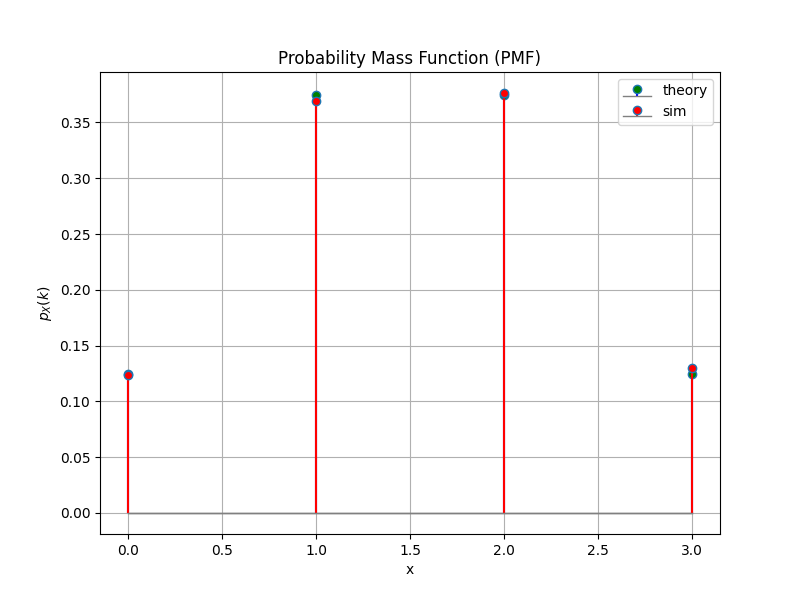
\includegraphics[width=\columnwidth]{figs/pmf.png}
    \caption{Probability Mass Function of given Random variable}
\end{figure}
\begin{figure}[h!]
   \centering
   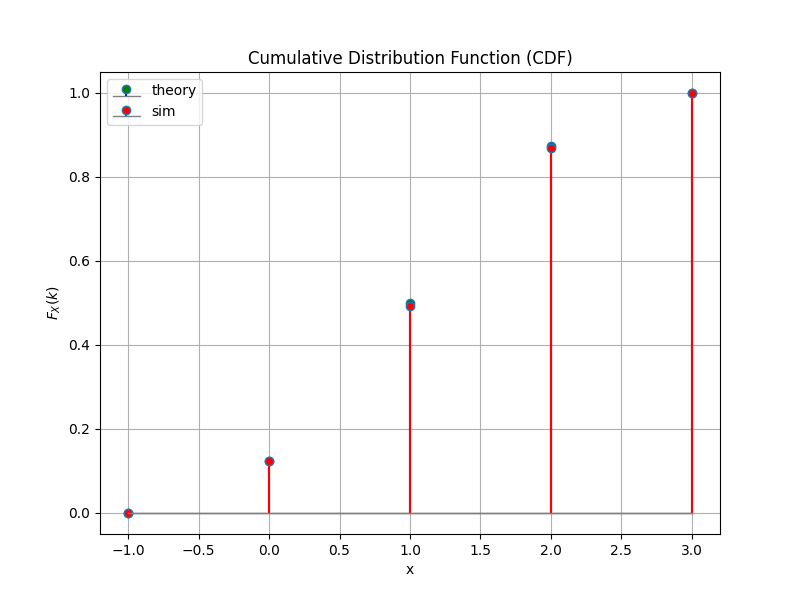
\includegraphics[width=\columnwidth]{figs/cdf.png}
    \caption{Cumulative Distribution Function of given Random variable}
\end{figure}
\end{enumerate}
\end{document}
